\documentclass[a4paper]{article}

\usepackage[english]{babel}
\usepackage[utf8x]{inputenc}
\usepackage{graphicx}
\usepackage{amsthm}
\usepackage{amssymb}
\usepackage{amsmath}
\usepackage{nicematrix}
\usepackage{tensor}
\usepackage{physics}
\usepackage{xcolor}
\usepackage{enumitem}
\usepackage{pgfplots}
\usepgfplotslibrary{fillbetween}

\usepackage[backend=biber,style=ieee,citestyle=numeric-comp,sorting=none]{biblatex}
\addbibresource{sample.bib}

\newtheorem{remark}{Remark}[section]
\newtheorem{definition}{Definition}[section]
\theoremstyle{definition}
\newtheorem{lemma}{Lemma}[section]
\newtheorem{theorem}{Theorem}[section]
\newtheorem{example}{Example}[section]
\newtheorem{corollary}{Corollary}[section]
\newtheorem{condition}{Assumption}[section]
\newtheorem{insight}{Insight}[section]
\newtheorem{problem}{Problem}[section]
\newtheorem*{solution}{Solution}

\title{Math Prep Course Day One}
\author{Ashhad}

\begin{document}

\maketitle

\section{Logic Exercises}
\begin{problem}
Truth table for \(P \land (Q \lor R) \iff (P \land Q) \lor (P \land R)\)
\end{problem}

Table for the left hand side

\[
\begin{array}{c|c|c|c|c}
P & Q & R & Q \lor R & P \land (Q \lor R) \\
\hline
T & T & T & T & T \\
T & T & F & T & T \\
T & F & T & T & T \\
T & F & F & F & F \\
F & T & T & T & F \\
F & T & F & T & F \\
F & F & T & T & F \\
F & F & F & F & F \\
\end{array}
\]

Table for the Right hand side

\[
\begin{array}{c|c|c|c|c|c}
P & Q & R & P \land Q & P \land R  & (P \land Q) \lor (P \land R) \\
\hline
T & T & T & T & T & T \\
T & T & F & T & F & T \\
T & F & T & F & T & T \\
T & F & F & F & F & F \\
F & T & T & F & F & F \\
F & T & F & F & F & F \\
F & F & T & F & F & F \\
F & F & F & F & F & F \\
\end{array}
\]

Final table
\[
\begin{array}{c|c|c}
P \land (Q \land R) &(P \land Q) \lor (P \land R) & P \land (Q \land R) \iff (P \land Q) \lor (P \land R)\\
\hline
T & T & T \\
T & T & T \\
T & T & T \\
F & F & T \\
F & F & T \\
F & F & T \\
F & F & T \\
F & F & T \\
\end{array}
\]

Thus the two logical statements are equivalent for all truth values.
\newpage
\begin{problem}
Prove or disprove
\[
\forall x \in \mathbb{R}, \ x^2 > 0
\]
\end{problem}
\begin{solution}
For the universal quantifier \(\forall\), a solution by contradiction is sufficient. We show that there exists an element \(x \in \mathbb{R}\) such that \(x^2 \ngtr 0\). 
\\ \\
Take \(x = 0\), then \(x^2 = 0 \ngtr 0\), and since we have \(\exists x \in \mathbb{R} , \ x^2 \ngtr 0\) then the statement \(\forall x \in \mathbb{R}, \ x^2 > 0\) cannot simultaneously hold, thus contradiction.
\end{solution}

\begin{problem}
Prove or disprove
\[
\forall n \in \mathbb{N}, \ n^2 > 2
\]
\end{problem}
\begin{solution}
Following the same pattern as last time, we choose the natural number \(n=1\) and obtain \(n^2 = 1 \ngtr 2\), thus obtaining our contradiction.
\end{solution}

\begin{problem} Prove or Disprove
\[
\forall x \in \mathbb{R}, \ \exists y, \ y< x
\]
\end{problem}
\begin{solution}
For any real number \(x \in \mathbb{R}\) we know that \(x-1\) is a well-defined real number. We also know that \(x-1 < x\). Therefore, for each real number \(x\), there exists at least the number \(y = x-1\) such that \(y < x\), thus the proposition holds true.
\end{solution}

\section{Set Operations}
\begin{problem}
Take the following sets
\begin{align*}
A &= \{-1, 0, 3, 4, 5, 6\} \\
B &= \{0, 1, 2, 3, 4\} \\
C &= \{0,2,4\} \\ 
\end{align*}
Find
\(A \cap C, \ A \cap B,  \ B \cap C, \ A \cap B \cap C\)
\end{problem}
\begin{solution}
\begin{align*}
A \cap B &= \{0,3,4\} \\
A \cap C &= \{0,4\} \\
B \cap C &= \{0,2,4\} \\
A \cap B \cap C &= \{0, 4\}
\end{align*}
\end{solution}

\newpage
\section{Summation and Product Formulae}
\begin{problem}
Evaluate
\[
\sum_{x=2}^4 (x^2-x)
\]
\end{problem}
\begin{solution}
Use \(x^2 -x = x(x-1)\)
Then our expression becomes via substitution
\begin{align*}
\sum_{x=2}^4 x(x-1) &= 2(2-1) + 3(3-1) + 4(4-1) \\
&= 2 + 6 + 12 \\
&=20
\end{align*}
\end{solution}

\begin{problem}
Evaluate
\[
\prod_{x=0}^5 x^2
\]
\end{problem}
\begin{solution}
Since \(0^2 = 0\), the first term \(x = 0\) reduces the entire product to zero. More formally we may write
\begin{align*}
\prod_{x=5}^5 x^2 &= 0^2 \times \prod_{x=1}^5x^2 \\ 
&= 0
\end{align*}
\end{solution}

\begin{problem}
Evaluate
\[
\prod_{x=1}^{4}x^2-(x-1)^2
\]
\end{problem}
\begin{solution}
Simplifying \(x^2 - (x-1)^2 = 2x -1\)
\begin{align*}
\prod_{x=1}^4 (2x-1) &= (2-1)(4-1)(6-1)(8-1) \\
&=105
\end{align*}
\end{solution}

\begin{problem}
Evaluate
\[
\sum_{x=1}^{100} x
\]
\end{problem}
\begin{solution}
This question is best solved with the aid of a useful and rather famous identity \(\sum_{x=1}^n = \frac{n(n+1)}{2}\). But if you think it is unfair to rely on prior knowledge consider this solution:
\begin{align*}
\sum_{x=1}^{100}x &= \sum_{x=1}^{49}x + \sum_{x=1}^{49}(100-x) + 50 + 100 \\
&= \sum_{x=1}^{49}100 + 150 \\
&= 5050
\end{align*}
\end{solution}

\section{Binomial Theorem}
\begin{problem}
Evaluate
\[
(10.1)^3
\]
\end{problem}
\begin{solution}
Expand the term inside the cube to \((10+0.1)^3\)
\begin{align*}
(10+0.1)^3 &= \sum_{i=0}^3 {i \choose 3} (10)^i(0.1)^{3-i} \\
&= \sum_{i=0}^3 {i \choose 3}(10)^i(10^{-1})^{3-i} \\
&= \sum_{i=0}^3 {i \choose 3}(10)^i(10)^{i-3} \\
&= \sum_{i=0}^3 {i \choose 3}(10)^{2i-3} \\
&= (10)^{-3} +3(10)^{-1} + 3(10) + (10)^3
\end{align*}
\end{solution}


\begin{problem}
Evaluate
\[
(99)^3
\]
\end{problem}
\begin{solution}
Expand the term inside the cube to \((100+(-1))^3\)
\begin{align*}
(100-1)^3 &= \sum_{i=0}^3 {i \choose 3} (100)^i(-1)^{3-i} \\
&= (-1)^{3} + 3(100)(-1)^2 + 3(100)^2(-1) + (100)^3
\end{align*}
\end{solution}

\section{Inequalities}
\begin{problem}
\[
\left| |x+2|-|x-2| \right| > 2
\]
\end{problem}
\begin{solution}
We begin by first splitting the intervals of \(|x+2|\) and \(|x-2|\) respectively to simplify the equation. Thus we obtain
\begin{align*}
|x+2| = 
\begin{cases}
    x+2, &x \geq -2 \\
    -x-2, &x \leq -2
\end{cases}
\end{align*}
Similarly
\begin{align*}
|x-2| = 
\begin{cases}
    x-2, &x \geq 2 \\
    2-x, &x \leq 2
\end{cases}
\end{align*}
Thus our intervals become \(\{(-\infty, -2], (-2, 2), \ [2, \infty)\} \).
Evaluating our functions on these intervals, we obtain
\begin{align*}
(-x-2) - (2-x) &= -4 & x \in (-\infty, -2] \\
(x+2) - (2-x) &= 2x & x \in (-2, 2) \\
(x+2) - (x-2) &= 4 & x \in [2, \infty)
\end{align*}
Notice that for the first and last case, the absolute value is always greater than 2. Therefore we direct our attention to the middle case where we impose the condition
\begin{align*}
|2x| &> 2 && x \in (-2, 2) \\
|x| &>  1
\end{align*}
The solutions to which in the interval \((-2, 2)\) are \((-2, -1)\) and \((1, 2)\).
\\ \\
Our solution set is therefore \((-\infty, -2] \cup (-2, -1) \cup (1, 2) \cup [2, \infty)\). Simplifying, we obtain
\[
(-\infty, -1) \cup (1, \infty)
\]

\begin{tikzpicture}
\begin{axis}[axis lines=middle, ymin=0, ymax=5, xmin=-5, xmax=5, width = 12cm, height =8cm, title={Individual graphs}]
\addplot[color=red, thick,]{-x-2};
\addplot[color=red, thick, dashed, domain=-1:1]{x+2};
\addplot[color=red, thick, domain=-5:-1]{x+2};
\addplot[color=red, thick, domain=1:5]{x+2};
\addplot[color=blue, thick,]{x-2};
\addplot[color=blue, thick, dashed, domain=-1:1]{2-x};
\addplot[color=blue, thick, domain=1:5]{2-x};
\addplot[color=blue, thick, domain=-5:-1]{2-x};
\addplot[color=gray, dashed] coordinates {(1,0) (1,3)};
\addplot[color=gray, dashed] coordinates {(-1,0) (-1,3)};
\end{axis}
\end{tikzpicture}

The blue line indicates the function \(|x-2|\) whilst the red indicates \(|x+2|\)

\begin{tikzpicture}
\begin{axis}[axis lines=middle, ymin=0, ymax=5, xmin=-5, xmax=5, width = 12cm, height =8cm, title={Graph of \(||x+2|-|x-2||\)}]
\addplot[color=blue, thick, domain=-5:-2]{4};
\addplot[color=blue, thick, domain=2:5]{4};
\addplot[color=red, thick, domain=1:2]{2*x};
\addplot[color=red, thick, domain=-2:-1]{-2*x};
\addplot[color=gray, dashed, thick, domain=-1:1]{2*x};
\addplot[color=gray, dashed, thick, domain=-1:1]{-2*x};
\addplot[color=gray, dashed] coordinates {(1,0) (1,2)};
\addplot[color=gray, dashed] coordinates {(-1,0) (-1,2)};
\end{axis}
\end{tikzpicture}

\end{solution}

\begin{problem}
\[
(x-3)(x+2)x < 0
\]
\end{problem}
\begin{solution}
The roots of the polynomial given are
\begin{align*}
x &= 0 \\
x+2 &= 0 \implies x = -2 \\
x-3 &= 0 \implies x = 3 \\
\end{align*}
Thus our intervals become \(\{(-\infty, -2), (-2, 0), (0, 3), (3, \infty)\}\)\footnote{We exclude the roots themselves since the polynomial is zero at those points and thus not less than zero as the condition requires}
Evaluating our polynomials on the following intervals we observe that
\begin{align*}
(x-3)(x+2)x < 0 &&x \in (-\infty, -2)
\end{align*}
Since all three terms are negative here, this interval satisfies our condition.
\begin{align*}
(x-3)(x+2)x < 0 &&x \in (-2, 0)
\end{align*}
Here only the \(x-3\) and \(x\) terms are negative, thus we have an overall positive evaluation. This interval does not satisfy our condition.
\begin{align*}
(x-3)(x+2)x < 0 &&x \in (0, 3)
\end{align*}
Since only the \(x-3\) term is negative, this interval too satisfies our condition.
\begin{align*}
(x-3)(x+2)x < 0 &&x \in (3, \infty)
\end{align*}
Beyond this point all our values are positive, thus our condition is not satisfied. The interval satisfying our requirement are therefore
\begin{align*}
(-\infty, -2) \cup (0, 3)
\end{align*}
\end{solution}

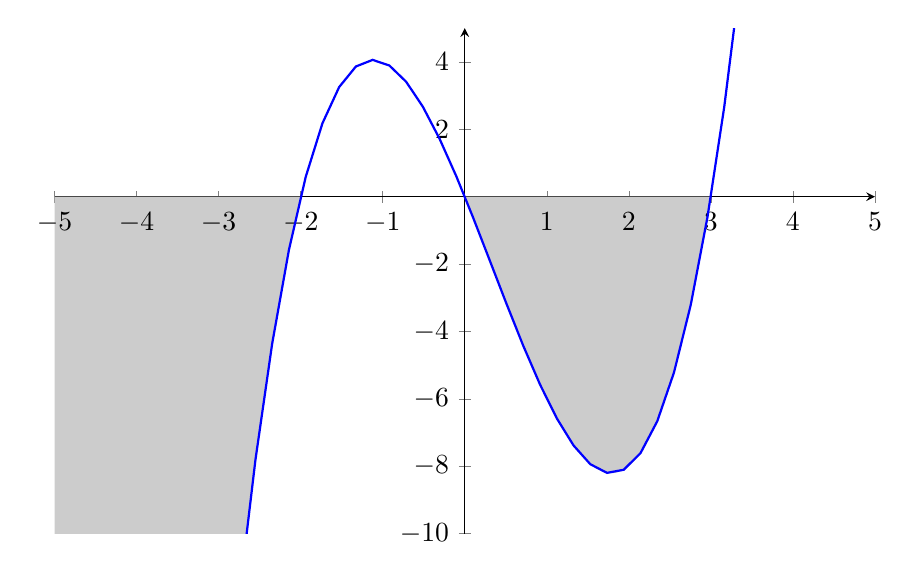
\begin{tikzpicture}
\begin{axis}[axis lines=middle, ymin=-10, ymax=5, xmin=-5, xmax=5, width = 12cm, height =8cm]
\addplot[color=blue, thick, samples=50]{(x-3)*(x+2)*x};
\addplot[name path=leftcurve, color=blue, thick, samples=50, draw=none, domain=-5:-2]{(x-3)*(x+2)*x};
\addplot[name path=rightcurve, color=blue, thick, samples=50, draw=none, domain=0:3]{(x-3)*(x+2)*x};
\addplot[name path=leftaxis, domain=-5:-2, draw=none] {0};
\addplot[name path=rightaxis, domain=0:3, draw=none] {0};
\addplot[gray!40] fill between[of=leftcurve and leftaxis];
\addplot[gray!40] fill between[of=rightcurve and rightaxis];
\end{axis}
\end{tikzpicture}

\newpage
\begin{problem}
\[
-2 < 1 - \frac{1}{x} < 0
\]
\end{problem}
\begin{solution}
Simplify the expression to \(-2 < \frac{x-1}{x} < 0\)
\begin{align*}
-2x < x -1 < 0 \\
2x > 1-x > 0 \\
\end{align*}
Since the final \(> 0\) condition ensures that \(1-x\) is positive, we can divide the equation by it without having to check for its signature. Therefore
\begin{align*}
\frac{2x}{1-x} > 1 > 0
\end{align*}
The last inequality is trivial so we omit it. We now check when \(\frac{2x}{1-x} > 1\) or rather, \(\frac{3x-1}{1-x} > 0\). Observe that \(1-x\) is positive on the domain \((-\infty, 1)\) and negative otherwise\footnote{We omit the point 1 since our expression is undefined at that point}, similarly \(3x-1\) is positive on the domain \((\frac{1}{3}, \infty)\) and negative otherwise. \\ 

All in all this gives us the three domains \(\{(-\infty, \frac{1}{3}), (\frac{1}{3}, 1), (1, \infty)\}\). Evaluating the expression we observe that 
\begin{align*}
\frac{3x-1}{1-x} && x \in \left(-\infty, \frac{1}{3}\right)
\end{align*}
The numerator is negative whilst the denominator is positive, thus this does not satisfy our condition.
\begin{align*}
\frac{3x-1}{1-x} && x \in \left(\frac{1}{3}, 1\right)
\end{align*}
The numerator is positive and so is the denominator, thus this interval satisfies our condition.
\begin{align*}
\frac{3x-1}{1-x} && x \in (1, \infty)
\end{align*}
Here, the numerator is positive but the denominator is negative, thus this interval too does not satisfy our condition.

The only interval is therefore 
\[
\left(\frac{1}{3}, 1\right)
\]

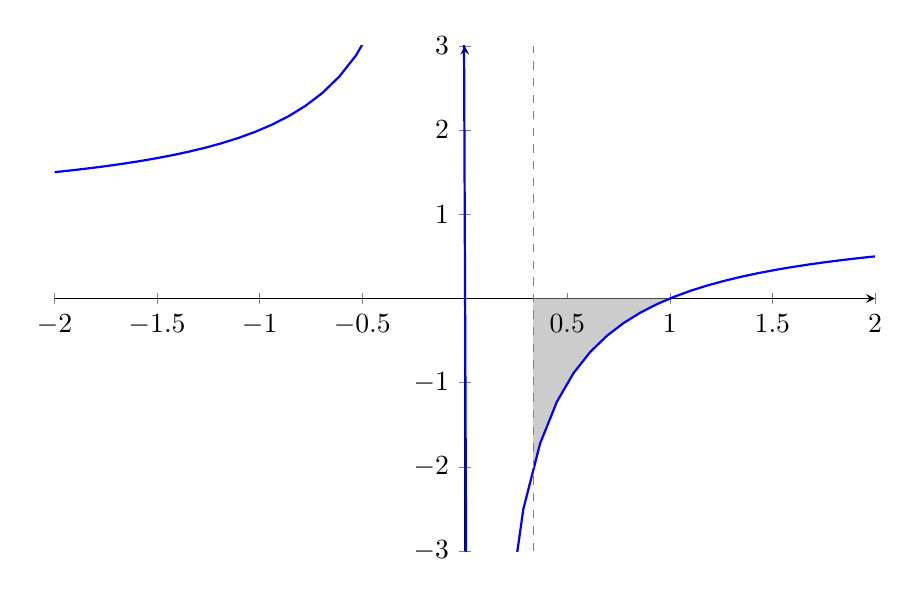
\begin{tikzpicture}
\begin{axis}[axis lines=middle, ymin=-3, ymax=3, xmin=-2, xmax=2, width = 12cm, height =8cm]
\addplot[color=blue, thick, samples=50, domain=-2:2]{1-1/x};
\addplot[name path=curve, color=blue, thick, samples=50, domain=0.3333:1, draw=none]{1-1/x};
\addplot[name path=axis, domain=0.3333:1, draw=none] {0};
\addplot[color=gray, dashed] coordinates {(0.3333, -3) (0.3333, 3)};
\addplot[gray!40] fill between[of=curve and axis];
\end{axis}
\end{tikzpicture}
\end{solution}
\end{document}
